\documentclass[12pt, a4]{article}
\usepackage[english]{babel}
\usepackage[utf8x]{inputenc}
\usepackage{fullpage}
\usepackage{listings}
\usepackage{graphicx}
\usepackage{color}

%Syntax highlighting
\definecolor{blue-violet}{rgb}{0.54, 0.17, 0.89}
\definecolor{ao}{rgb}{0.0, 0.5, 0.0}
\definecolor{amaranth}{rgb}{0.9, 0.17, 0.31}
\definecolor{ballblue}{rgb}{0.13, 0.67, 0.8}
\definecolor{onyx}{rgb}{0.06, 0.06, 0.06}


\lstset{
  breaklines=true,                 % automatic line breaking only at whitespace
  captionpos=b,                    % sets the caption-position to bottom
  breakatwhitespace=false,
  keepspaces=true,
  numbers=left,
  numbersep=5pt,
  showspaces=false,
  showstringspaces=false,
  showtabs=false,
  tabsize=4,  
  backgroundcolor=\color{white},   % choose the background color
  commentstyle=\color{ao},    % comment style
  keywordstyle=\color{amaranth},    % keyword style
  stringstyle=\color{blue-violet},    % string literal style
  numberstyle=\tiny\color{ballblue},	   % number style
  basicstyle=\ttfamily\footnotesize\color{onyx} % size of fonts used for the code
}

%Document Header
\title{\textbf{Department of CSE\\SSN College of Engineering}}
\author{\textbf{Vishakan Subramanian - 18 5001 196 - Semester VII}}
\date{09 August 2021}

\begin{document}
\maketitle
\hrule
\section*{\center{UCS 1712 - Graphics And Multimedia Lab}}
\hrule
\bigskip

%Assignment Details
\subsection*{\center{\textbf{Exercise 4: Midpoint Circle Drawing Algorithm in C++ using OpenGL}}}
\subsection*{\flushleft{Aim:}}
\begin{flushleft}
a) To plot points that make up the circle with center (xc,yc) and radius r using Midpoint circle drawing
algorithm. Give atleast 2 test cases.

\begin{itemize}
\item Case 1: With center (0,0)
\item Case 2: With center (xc,yc)
\end{itemize}

b) To draw any object using line and circle drawing algorithms. 
\newline
\newline
 
\end{flushleft}

%Code
\newpage
\subsection*{\flushleft{Code: Midpoint Circle Drawing Algorithm:}}
\begin{flushleft}
\lstinputlisting[language = C++]{MidpointCircle/main.cpp}
\end{flushleft}


%Output
\newpage
\subsection*{\flushleft{Output: Midpoint Circle Case 1 - C(400, 400) R - 200:}}
\begin{figure}[h]
\centering
\caption{Output: Midpoint Circle Case 1 - C(400, 400) R - 200.}
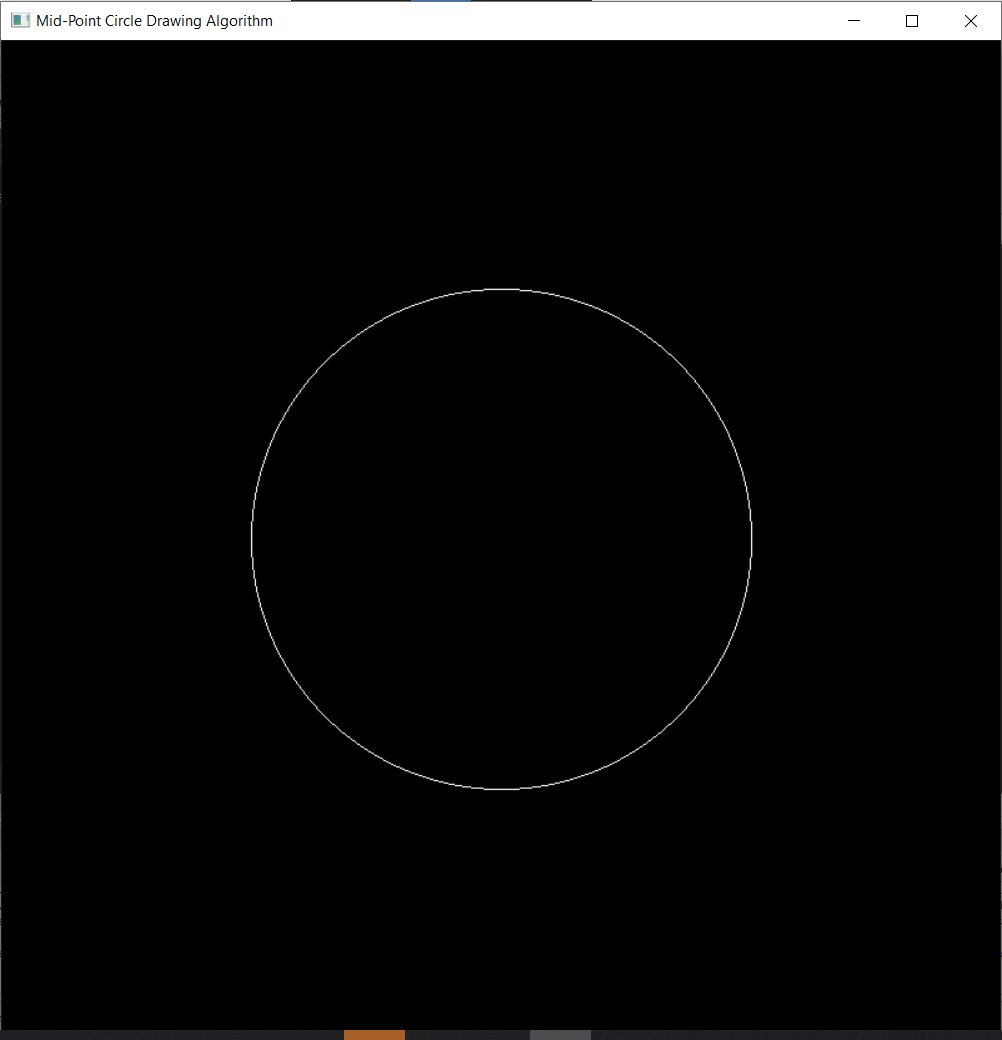
\includegraphics[height=15cm, width=15cm]{MidpointCircle/Outputs/Circle-1.png}
\end{figure}

%Output
\newpage
\subsection*{\flushleft{Output: Midpoint Circle Case 2 - C(200, 300) R - 50:}}
\begin{figure}[h]
\centering
\caption{Output: Midpoint Circle Case 2 - C(200, 300) R - 50.}
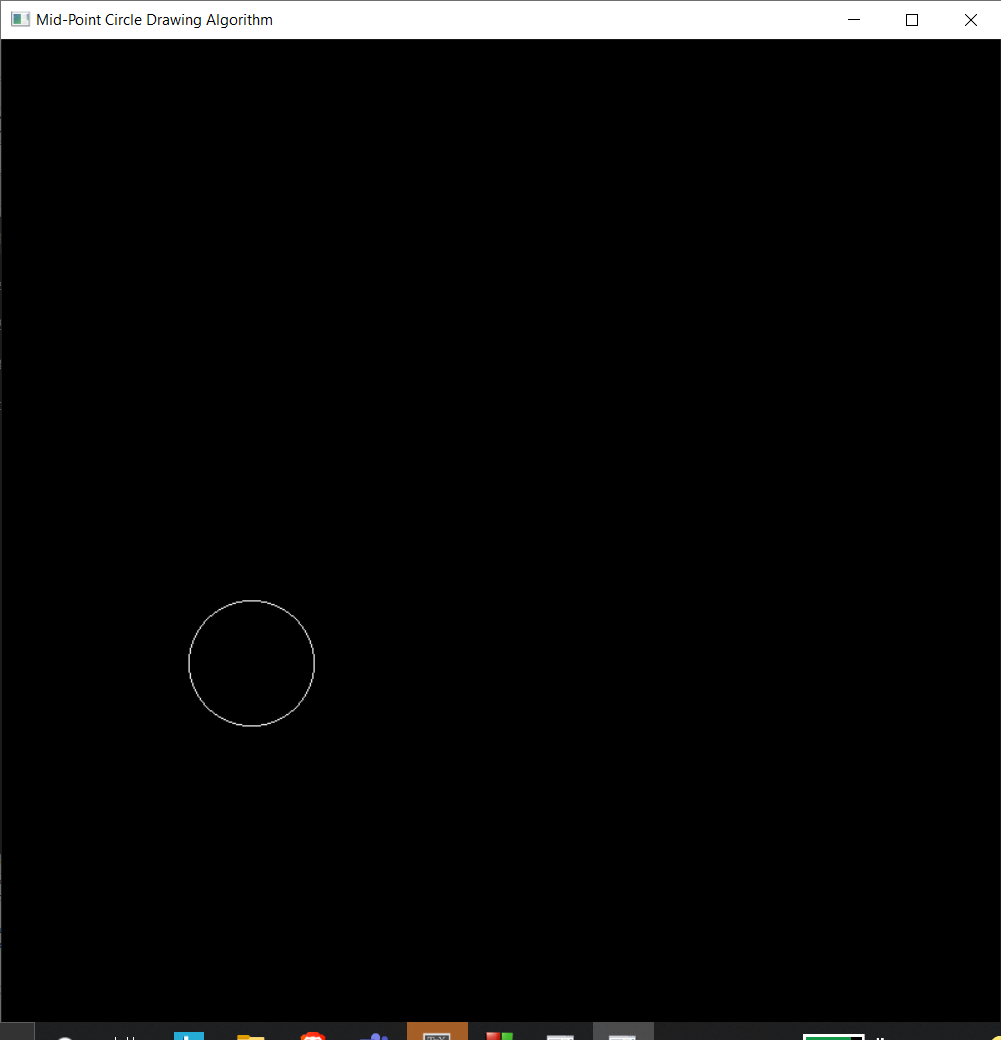
\includegraphics[height=15cm, width=15cm]{MidpointCircle/Outputs/Circle-2.png}
\end{figure}

%Code
\newpage
\subsection*{\flushleft{Code: Object Using Circles and Lines:}}
\begin{flushleft}
\lstinputlisting[language = C++]{Hangman/main.cpp}
\end{flushleft}

%Output
\newpage
\subsection*{\flushleft{Output: Stickman:}}
\begin{figure}[h]
\centering
\caption{Output: Stickman.}
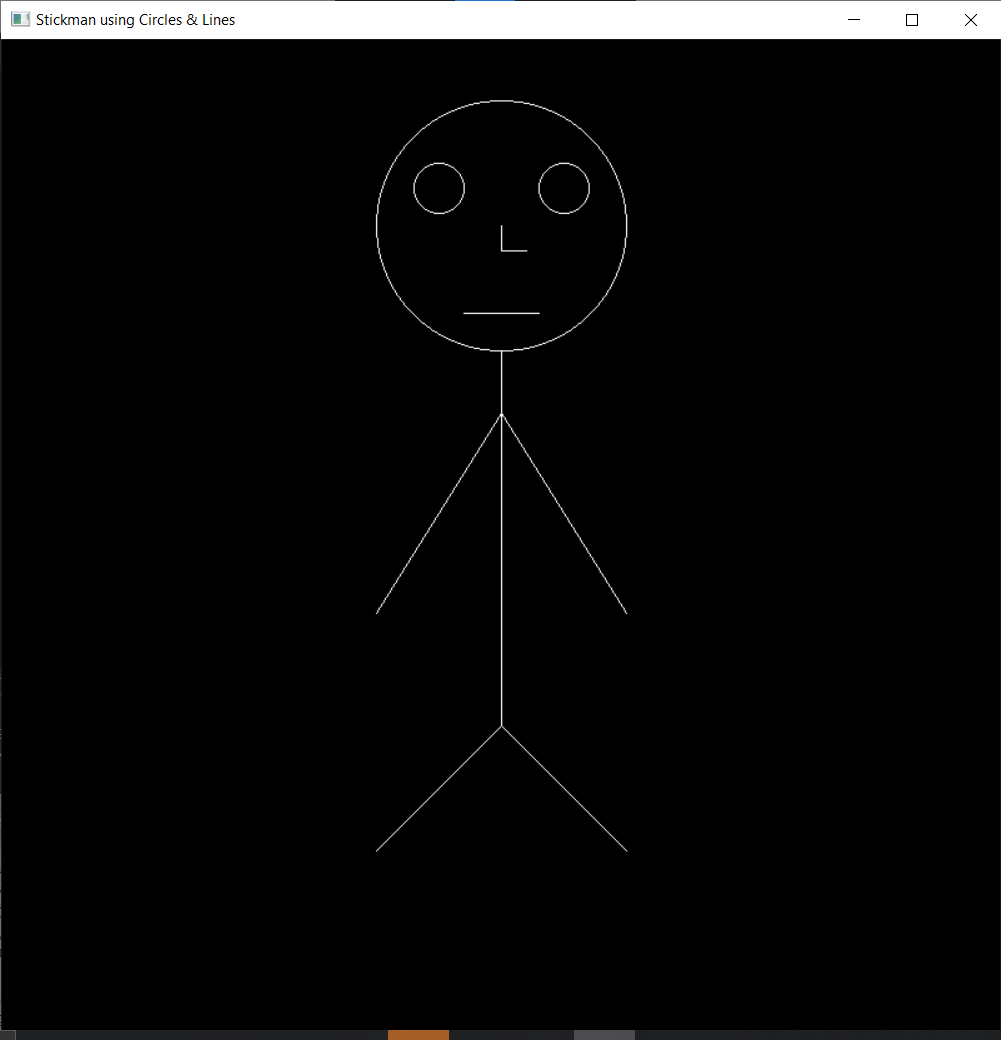
\includegraphics[height=15cm, width=15cm]{Hangman/Outputs/Stickman.png}
\end{figure}



%Learning Outcome
\newpage
\subsection*{\flushleft{Learning Outcome:}}
\begin{itemize}
\item I understood the \textbf{Midpoint Circle Drawing Algorithm}'s working.
\item I implemented the Midpoint Circle Drawing algorithm using an OpenGL program.
\item I understood how the algorithm makes use of \textbf{octant symmetry} and plots points on the second octant and mirrors it to other octants.
\item I understood how the parameter \textbf{p} is calculated in each iteration to determine the decrement of Y coordinate.
\item I learnt about \textbf{classes and member functions} in C++ to implement methods to facilitate the circle drawing algorithm process.
\item I was able to output all different test cases appropriately to verify the correctness of my program to implement the Midpoint Circle Drawing Algorithm.
\item I was able to draw and output a \textbf{Stickman} using the \textbf{Midpoint Circle Drawing Algorithm} and the \textbf{Bresenham's Line Drawing Algorithm}.

\end{itemize}


\end{document}